\documentclass{article}
\usepackage[utf8]{inputenc}
\usepackage{graphicx}
\usepackage{geometry}
\usepackage{hyperref}
\usepackage{indentfirst}
\usepackage{soul}
\usepackage{float}
\geometry{a4paper, total={170mm,257mm}, left=25mm, top=20mm, right=25mm, bottom=20mm}

\title{Cheems vs Sanity}
\author{Sayam Sethi (2019CS10399)\\Shrey Patel (2019CS10400)\\Rishi Shah (2019CS10395)}
\date{November, 2021}

\begin{document}

\maketitle

\tableofcontents

\newpage

\begin{abstract}
    Nowadays, memes are very popular throughout the Internet. They are used to express feelings, like happiness, anger, or sadness. They have become one of the most dominant forms of communication in the digital age and possibly the most favourite pastime of the younger generation. The beauty of a meme is that it is not just a picture, but a story. The story is the main content of the meme, and the story is the main reason for the popularity of the meme. And another feature of memes, that results from the larger context of the memes,  is that more often than not, they are interpreted differently by different people. Due to this, sometimes, even a single meme, which is nothing more than a piece of image or text, becomes a recurrent topic of discussion, as evident from the thousands of comments following some of the more popular memes on Reddit or Instagram.

    Following this reasoning, we will try and analyze the effect memes have on language. We use the meme language \textbf{Cheems} for our case study. We intend to delve deep in the origin, history, and usage of the language and also try to understand the usage of the language in the context of the memes. We will also discuss the evolution of the language among the community using various conversational examples and try to put forth various opinions of different language groups on the validity of the language.

    The above discussion is significant because it reflects on the development of languages in short term, and highlights the importance of digital media in this day and age and the impact it has shown on our community as a whole. We will try to show that the technology of today has played a pivotal role in truly turning the world into a global village, and we speculate that this study will give us an insight on the future development of languages or atleast what we can expect going forward.
\end{abstract}

\section{Theoretical Framework}
Normally, a particular language develops and evolves over hundreds and possibly thousands of years, for it to seep through a wide and diverse range of language communities. Most of the traditional languages like Hindi, Gujarati, English, etc. have been spread and passed upon, more or less through direct human communication and have been used in the past for a long time.  The prevalence which these languages have achieved is primarily because it has been passed and propogated through a variety of media like human speech and interaction, writing in the form of print media. But note that the biggest hindrance to the rapid spread of these languages is the sense of locality. The geographical barriers have caused the language spread to be abysmally slow and gradual.

However, the digital media today has caused information to flow much faster, regardless of barriers. So, nowadays, people are quicker to adapt to various cultural (especially related to language) and technological trends and concepts as compared to the past. People today are much more likely to be aware of affairs and incidents happening in different parts of the world. The teenagers today use a whole array of web jargon which supposedly makes them appear "cool" among their peers, like \textit{lol} (laugh out loud), \textit{gg} (good game), \textit{brb} (be right back) and so on. And what's fascinating is that all these web jargon then becomes a part of their daily language as well. It is not uncommon to come across who prefers to actually speak \textit{lol} instead of actually laughing at some joke or humorous remark. Another surprising fact about these internet "lingo" (pun totally intended) is that its users don't actually go through any sort of training or learning process. It's just practice through usage. No rules, no bounds, only usage. The surprising fluency may be because these are generally derived from a parent language, mostly English, but may be extended to other languages as well or due to the fact that the users of this language are quite frequently exposed to the usage of this kind of abbreviated language in different parts of the net. The constant exposure seems to be the better reason for the rapid growth in its users. 
    
Memes play a kind of a unique role in propogating this information. One might ask that online educational portals, blogs or research papers that are freely available throughtout the Internet should be the primary sources of intellectual ideas and concepts, and they are, to a large extent, but the painful reality is that most of us are often not patient or curious enough to dig through scores of \st{bland} text to get our daily dose of brain food. Most of us won't even log onto the Internet intending to learn something new but just to have fun or kill some time. Memes come to rescue in this scenario. They are fun, witty, and informative (mostly). Many times, they mock some stereotyped belief using hilarious examples or situations, or depict raging and controversial topics in a light-hearted manner. 

But the general view among the \st{boomers} digitally innocent generation is that the memes are a useless waste of time, that fill the brain with twisted and unconventional ideals and that they are another one of those undesirable outcomes when you give the youngsters too much freedom of speech and expression. But, memes are much more than just mere social media posts, they are a part of digital culture. Let's take an example. Consider the following meme:

\begin{figure}[H]
    \centering
    
\includegraphics[width=0.4\textwidth]{figures/meme1.png}
    \caption{A typical Internet meme}
\end{figure}

Now, the above meme has two visible humorous elements. One is exploiting the similarity between the spellings of ac-tor and doc-tor to create a sense of contrast. And the other, more intellectual one, is the satire on Indian education in which the meme refers to the situation in which a child conveys his dream/wish of becoming an actor to his father, but the stereotypical Indian father only considers being a doctor (or an engineer :) ) to be a good job, since they are usually the most respected/highly paid jobs in the country.So, in a satirical way, this meme portrays the state of Indian education and economy, though exaggerated, to the rest of the world, since the Indian culture has historically been the one which signifies hard work, skill, progress and innovation. However, this doesn't mean that the Indian culture has ever undermined or ignored talents in other fields like art, music, design, etc. 
\subsection{Origin and Etymology of Cheems}
Before \textbf{Cheems} became famous, a certain set of memes called \textbf{doge memes} rose to prominence. The word \textbf{doge} is a misspelling of the word \textit{dog}. One of the initial versions of the meme is:
\begin{figure}[H]
    \centering
    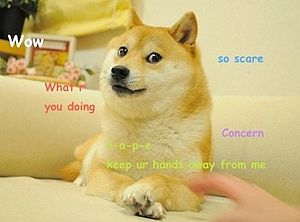
\includegraphics[width=0.5\textwidth]{figures/original_doge_meme.jpg}
    \caption{Original Doge Meme}
\end{figure}

As can be clearly seen from the meme, even though the language is still English, the way the phrases are structured gives it a very different feeling. Additionally, the phrases are terse and they don't follow the regular English grammar. In a way, the words use their root form instead of using the contextual morphemes. Another example of a meme of this category is:
\begin{figure}[H]
    \centering
    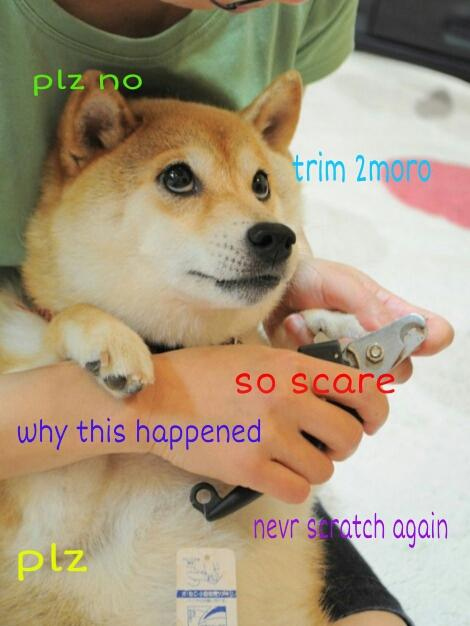
\includegraphics[width=0.3\textwidth]{figures/doge_2.jpg}
    \caption{Another example of the \textit{doge meme}}
\end{figure}

Again as we can see, the meme aims to convey a story without using too many words and it has the \textit{doge} flavour of English. The story being narrated is as follows:
\begin{itemize}
    \item The dog is requesting its master to not do something
    \item We then find out that the dog is requesting the master to trim its nails the next day
    \item The dog conveys that it is scared
    \item They also wonder why the master has decided to trim their nails
    \item They conclude that the master is trimming their nails because they scratched someone and hence promise that they will never scratch again
    \item The meme then ends with the dog requesting again
\end{itemize}


\subsubsection{Origin of the Doge Dog}



\section{Examples from Data}

\section{Problems of Fit}

\section{Conclusion}

\section{Notes and References}
% https://knowyourmeme.com/memes/doge
    

\end{document}